\chapter{Kanban Setup \\
\small{\textit{-- Tamara Gonzalez Ibarra}}
\index{Kanban Setup} 
\index{Chapter!Kanban Setup}
}
\label{Chapter::KanbanSetup}

In this chapter, I describe the steps I followed to set up a Kanban board with my group members in Trello. 
The purpose of the Kanban setup is to create a clear and visual workflow that helps manage tasks and track progress effectively for agile projects. 

\section{Creating the Board}
\begin{enumerate}
    \item Logged into Trello with my account.
    \item Clicked on \texttt{Create new board}.
    \item Named the board \textit{Kanban Board}, used a Kanban Board template, and selected a background for better visualization.
\end{enumerate}

\section{Setting Up Lists}
\begin{enumerate}
    \item Created the following lists to represent the workflow:
    \begin{itemize}
        \item \textbf{Backlog} – ideas and tasks that still need to be planned or refined.
        \item \textbf{Design} – tasks related to planning and designing before implementation.
        \item \textbf{To Do} – tasks that need to be started.
        \item \textbf{Doing} – tasks that are currently in progress.
        \item \textbf{Code Review} – tasks that are finished but require peer review before proceeding.
        \item \textbf{Testing} – tasks that have passed review and need to be tested for quality assurance.
        \item \textbf{Done} – completed tasks.
        
    \end{itemize}
    \item Ensured the lists followed left-to-right order.
\end{enumerate}

\begin{figure}[h!]
    \centering
    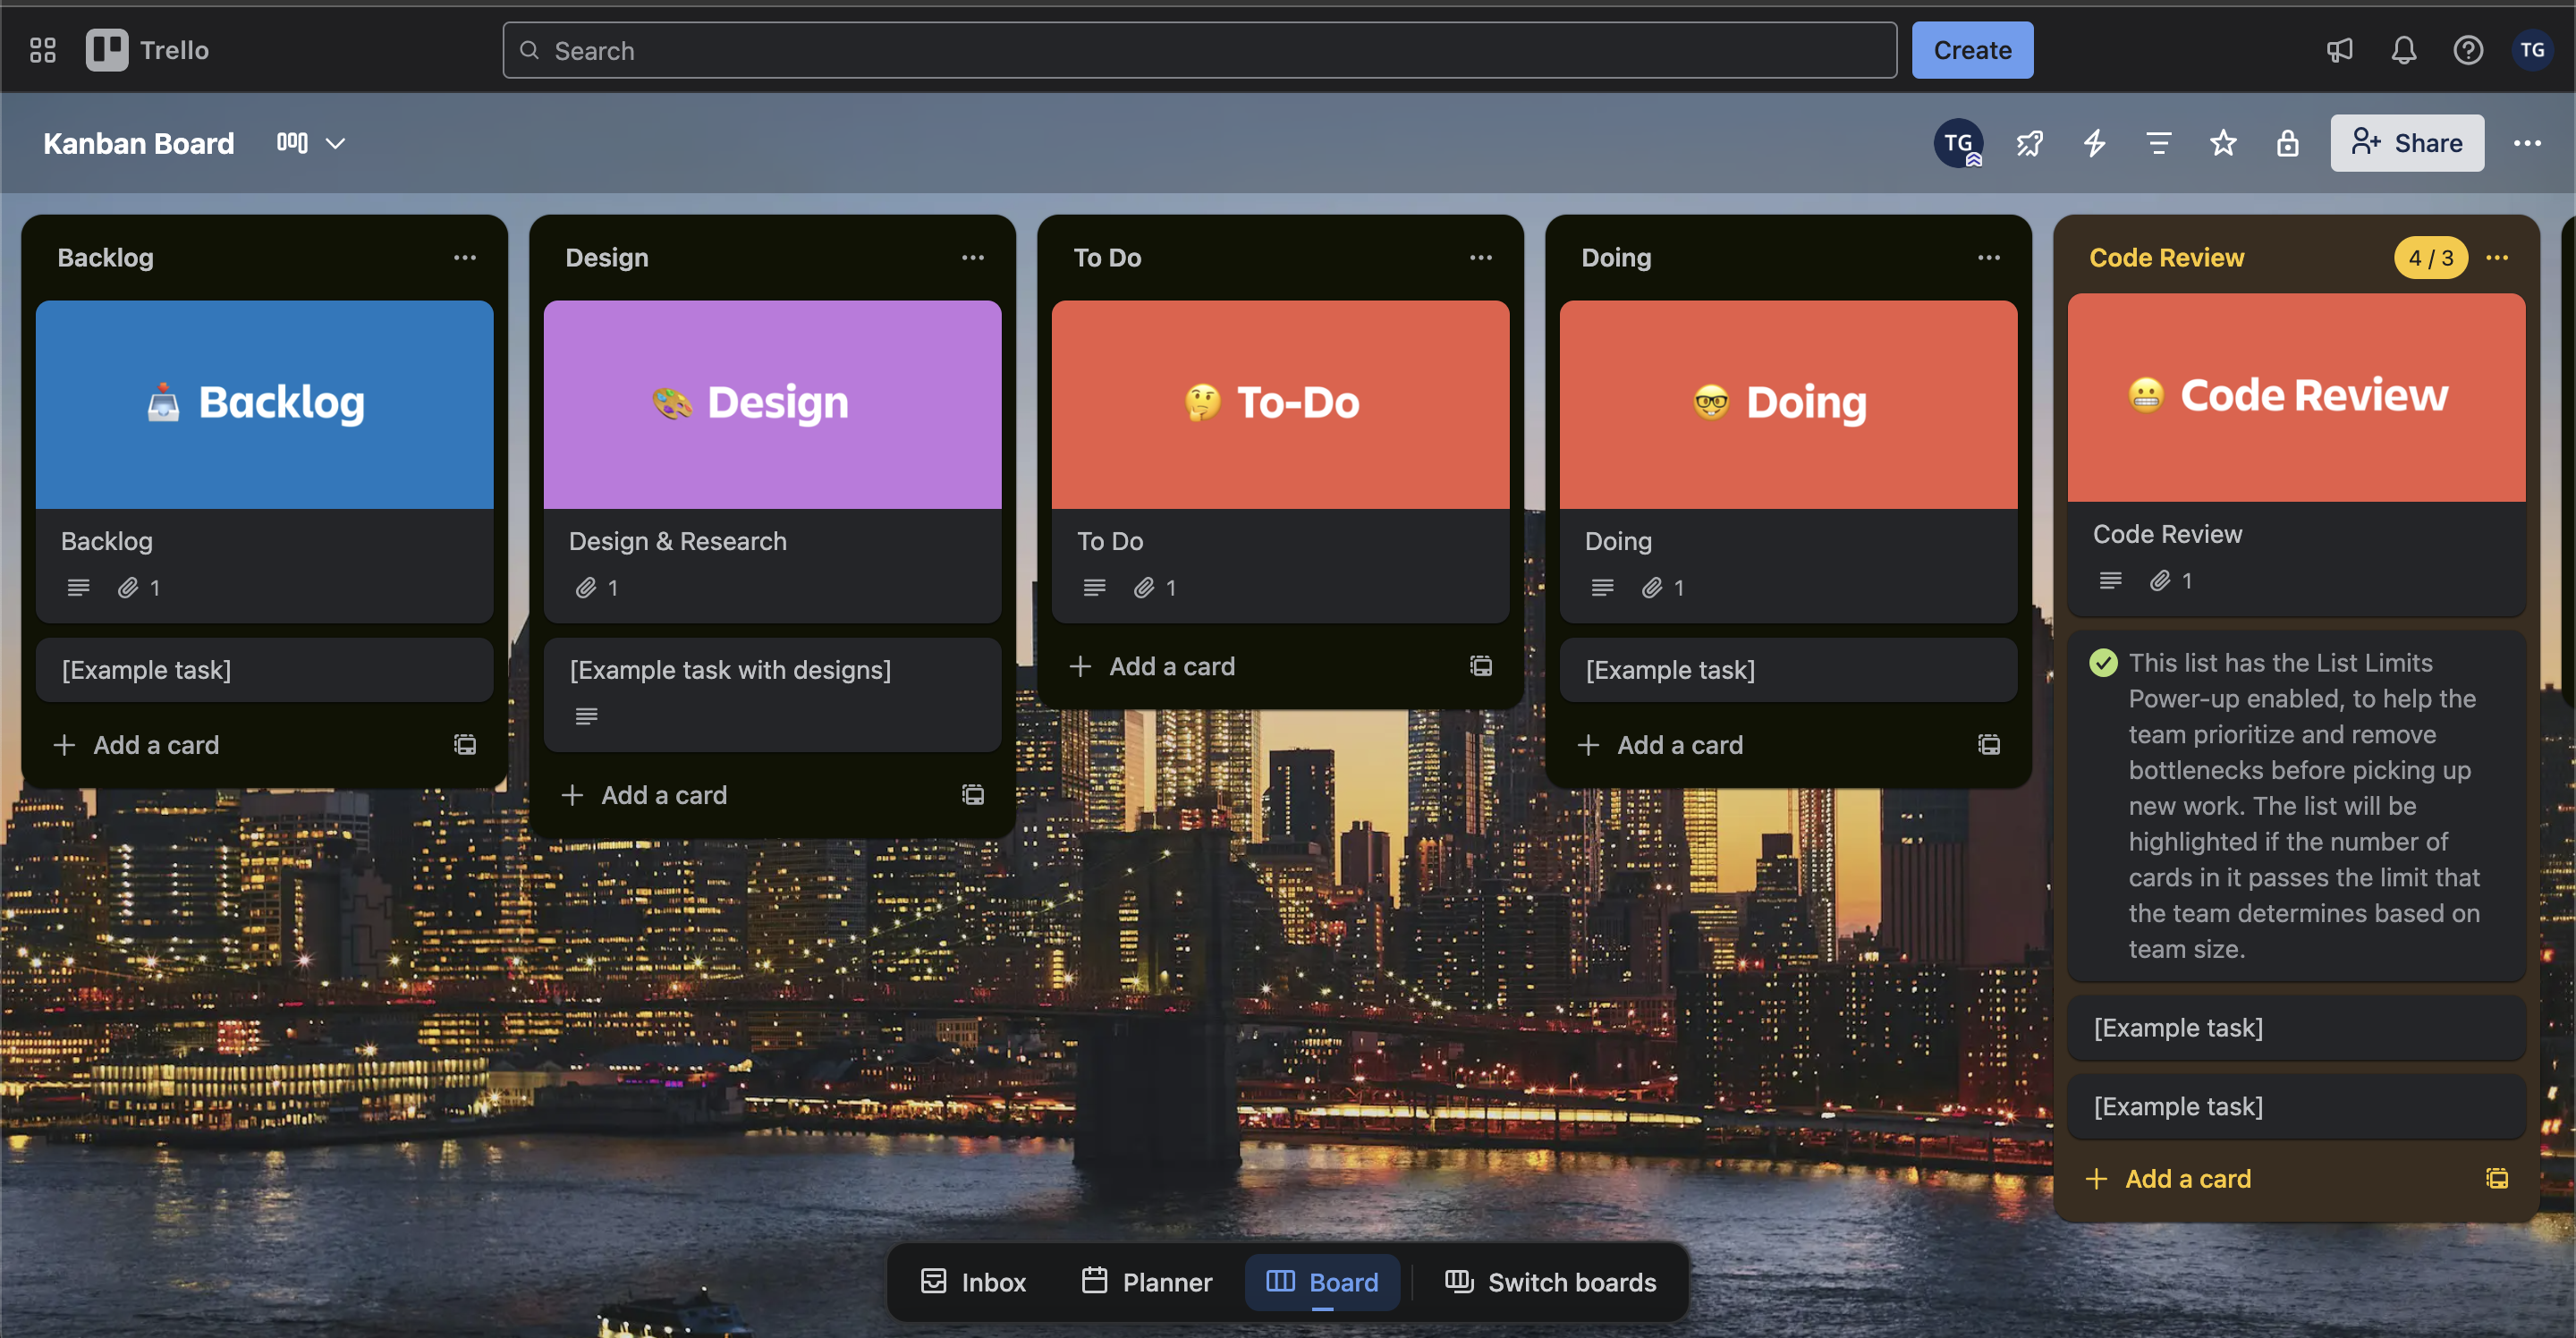
\includegraphics[width=0.8\textwidth]{kanban_board.png}
    \caption{Screenshot of the first half of Kanban Board in Trello.}
    \label{fig:kanban_board}
    
    \vspace{0.5cm} % space between images
    
    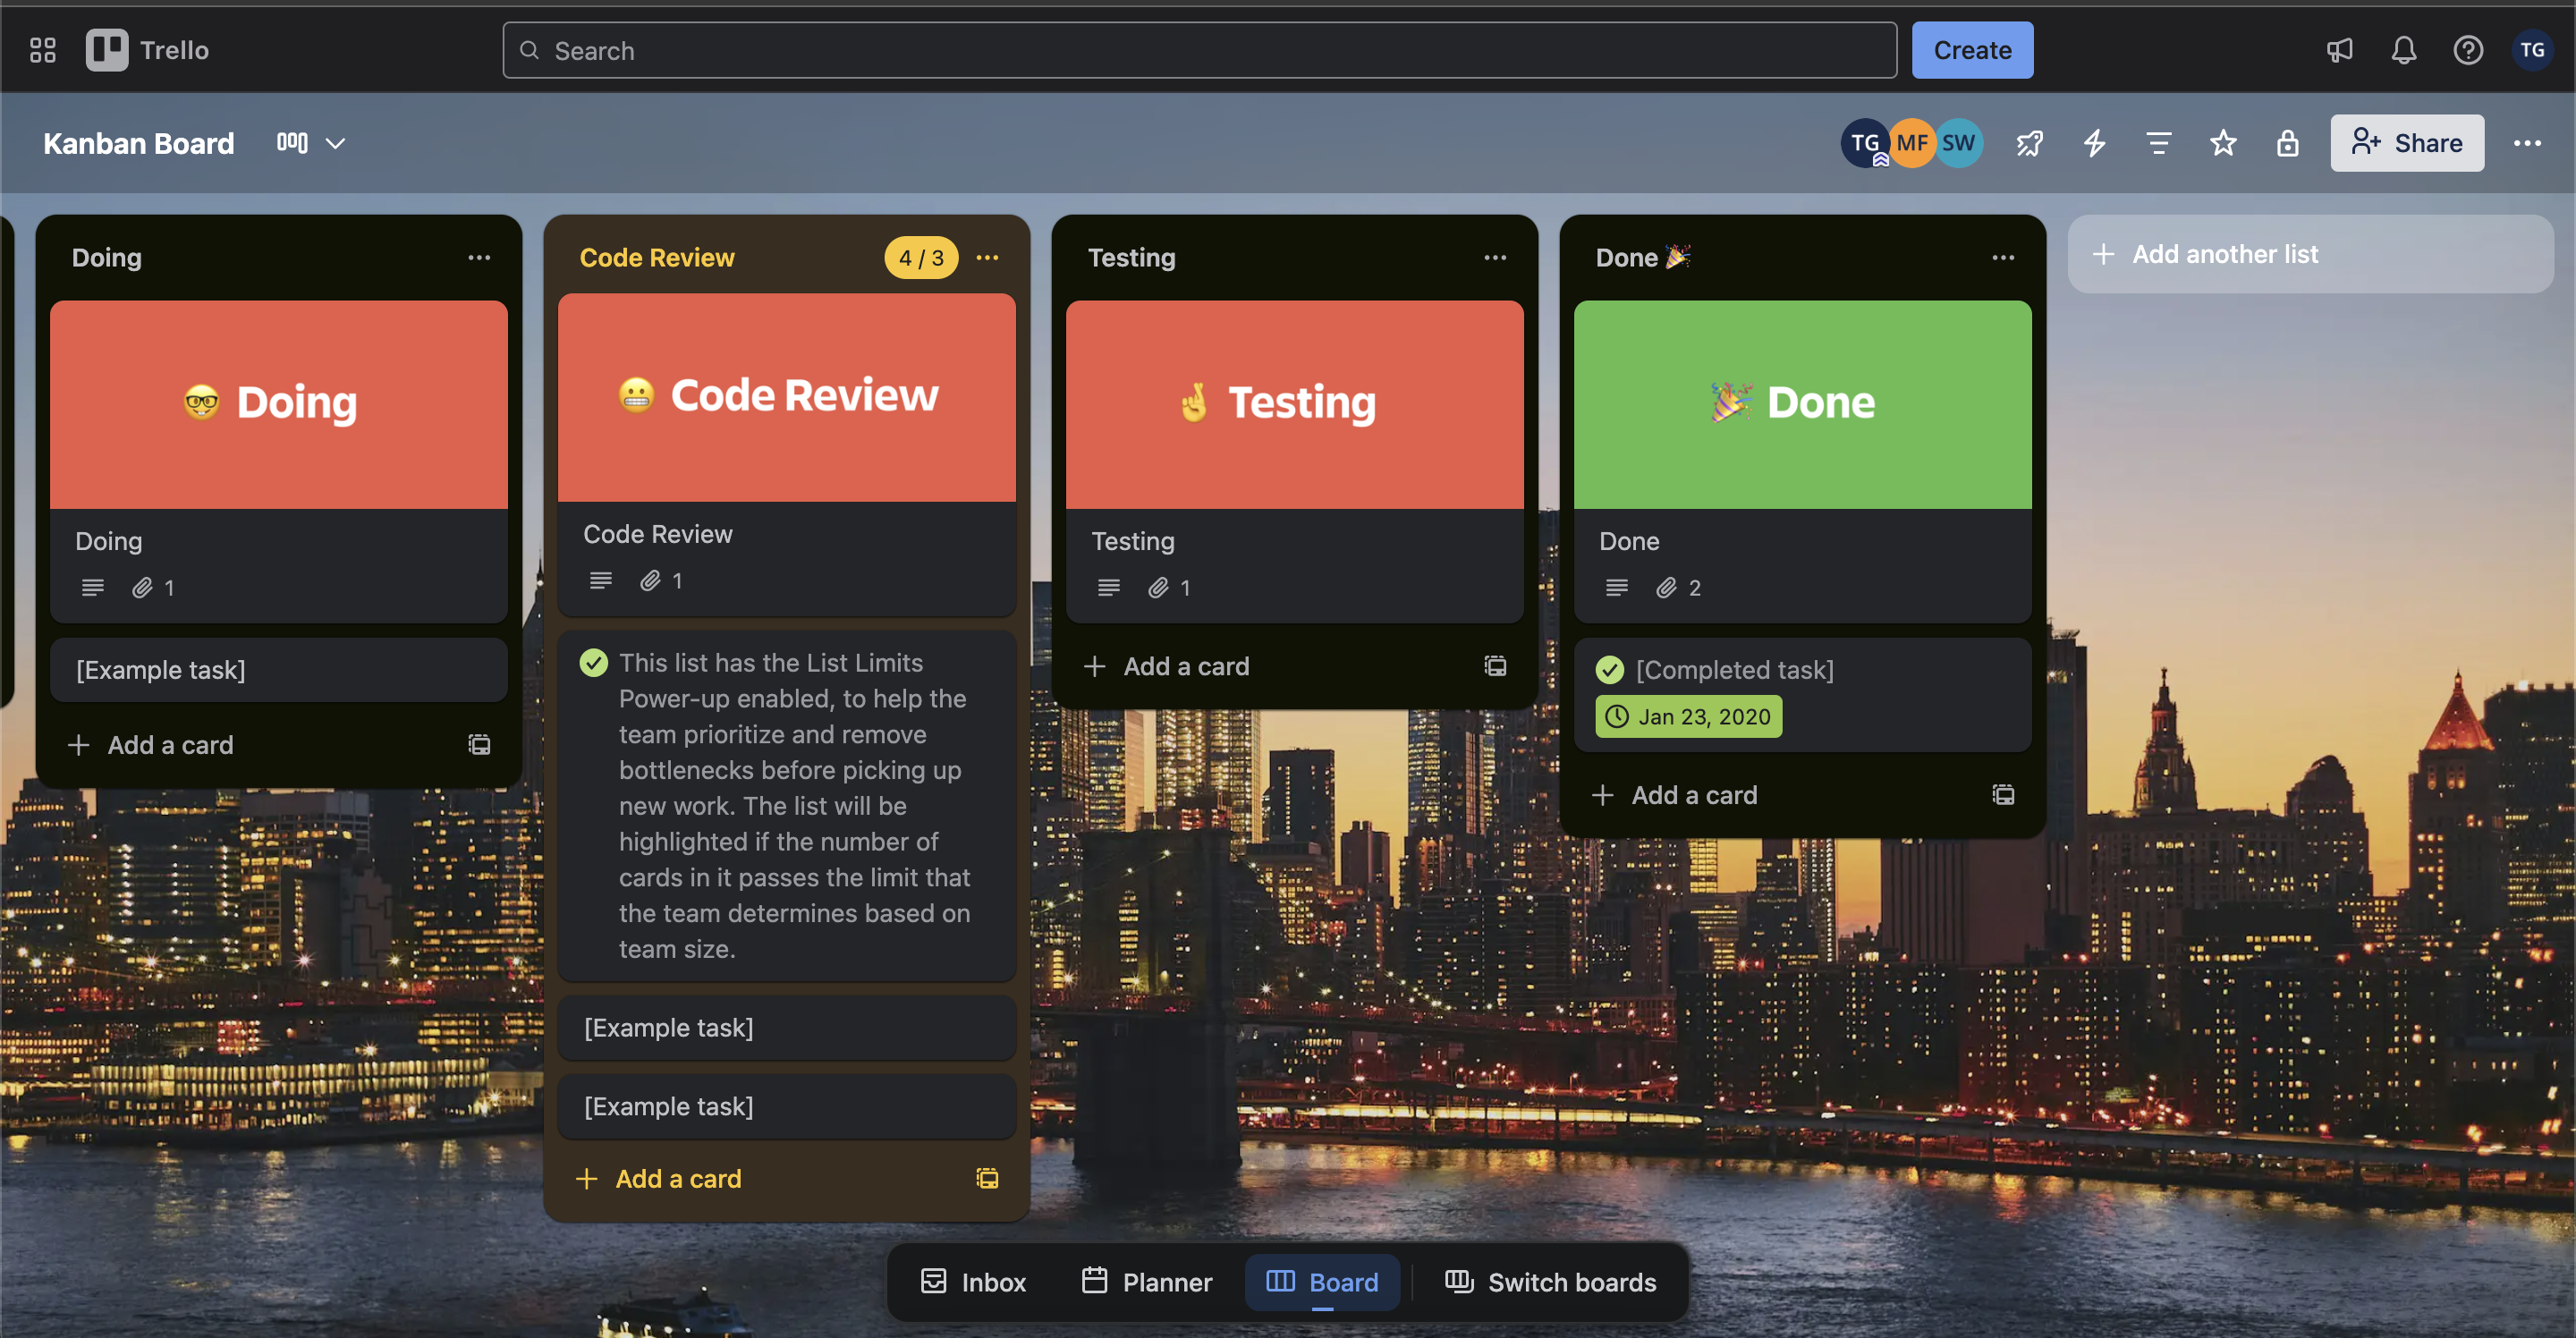
\includegraphics[width=0.8\textwidth]{kanban_board2.png}
    \caption{Screenshot of the second half of Kanban Board in Trello.}
    \label{fig:kanban_board2}
\end{figure}


\section{Using Trello Features}
\begin{enumerate}
    \item Enabled checklists within cards to track smaller subtasks.
    \item Attached files and links directly to cards for reference.
    \item Used Trello’s built-in automation (Butler) to move cards between lists when certain conditions were met (e.g., when a task is marked complete).
\end{enumerate}

This Kanban setup provides a clear structure for a future project to manage work and make it easier to track progress and stay organized throughout the project.
